\documentclass[bachelor, och, labwork]{shiza}
% параметр - тип обучения - одно из значений:
%    spec     - специальность
%    bachelor - бакалавриат (по умолчанию)
%    master   - магистратура
% параметр - форма обучения - одно из значений:
%    och   - очное (по умолчанию)
%    zaoch - заочное
% параметр - тип работы - одно из значений:
%    referat    - реферат
%    coursework - курсовая работа (по умолчанию)
%    diploma    - дипломная работа
%    pract      - отчет по практике
% параметр - включение шрифта
%    times    - включение шрифта Times New Roman (если установлен)
%               по умолчанию выключен
\usepackage{subfigure}
\usepackage{tikz,pgfplots}
\pgfplotsset{compat=1.5}
\usepackage{float}

%\usepackage{titlesec}
\setcounter{secnumdepth}{4}
%\titleformat{\paragraph}
%{\normalfont\normalsize}{\theparagraph}{1em}{}
%\titlespacing*{\paragraph}
%{35.5pt}{3.25ex plus 1ex minus .2ex}{1.5ex plus .2ex}

\titleformat{\paragraph}[block]
{\hspace{1.25cm}\normalfont}
{\theparagraph}{1ex}{}
\titlespacing{\paragraph}
{0cm}{2ex plus 1ex minus .2ex}{.4ex plus.2ex}

% --------------------------------------------------------------------------%


\usepackage[T2A]{fontenc}
\usepackage[utf8]{inputenc}
\usepackage{graphicx}
\graphicspath{ {./images/} }
\usepackage{tempora}

\usepackage[sort,compress]{cite}
\usepackage{amsmath}
\usepackage{amssymb}
\usepackage{amsthm}
\usepackage{fancyvrb}
\usepackage{listings}
\usepackage{listingsutf8}
\usepackage{longtable}
\usepackage{array}
\usepackage[english,russian]{babel}

% \usepackage[colorlinks=true]{hyperref}
\usepackage{url}

\usepackage{underscore}
\usepackage{setspace}
\usepackage{indentfirst} 
\usepackage{mathtools}
\usepackage{amsfonts}
\usepackage{enumitem}
\usepackage{tikz}

\newcommand{\eqdef}{\stackrel {\rm def}{=}}
\newcommand{\specialcell}[2][c]{%
\begin{tabular}[#1]{@{}c@{}}#2\end{tabular}}

\renewcommand\theFancyVerbLine{\small\arabic{FancyVerbLine}}

\newtheorem{lem}{Лемма}

\begin{document}

% Кафедра (в родительном падеже)
\chair{}

% Тема работы
\title{Инкапсуляция пакетов}

% Курс
\course{2}

% Группа
\group{231}

% Факультет (в родительном падеже) (по умолчанию "факультета КНиИТ")
\department{факультета КНиИТ}

% Специальность/направление код - наименование
%\napravlenie{09.03.04 "--- Программная инженерия}
%\napravlenie{010500 "--- Математическое обеспечение и администрирование информационных систем}
%\napravlenie{230100 "--- Информатика и вычислительная техника}
%\napravlenie{231000 "--- Программная инженерия}
\napravlenie{100501 "--- Компьютерная безопасность}

% Для студентки. Для работы студента следующая команда не нужна.
% \studenttitle{Студентки}

% Фамилия, имя, отчество в родительном падеже
\author{Окунькова Сергея Викторовича}

% Заведующий кафедрой
% \chtitle{} % степень, звание
% \chname{}

%Научный руководитель (для реферата преподаватель проверяющий работу)
\satitle{ассистент} %должность, степень, звание
\saname{А. А. Фомин}

% Руководитель практики от организации (только для практики,
% для остальных типов работ не используется)
% \patitle{к.ф.-м.н.}
% \paname{С.~В.~Миронов}

% Семестр (только для практики, для остальных
% типов работ не используется)
%\term{8}

% Наименование практики (только для практики, для остальных
% типов работ не используется)
%\practtype{преддипломная}

% Продолжительность практики (количество недель) (только для практики,
% для остальных типов работ не используется)
%\duration{4}

% Даты начала и окончания практики (только для практики, для остальных
% типов работ не используется)
%\practStart{30.04.2019}
%\practFinish{27.05.2019}

% Год выполнения отчета
\date{2021}

\maketitle

% Включение нумерации рисунков, формул и таблиц по разделам
% (по умолчанию - нумерация сквозная)
% (допускается оба вида нумерации)
% \secNumbering

%-------------------------------------------------------------------------------------------


\begin{enumerate}
    
    \item Воспользуйтесь сетью, настроенной вами в ходе выполнения работы №5.  Загрузите её 
    в ПакетТрейсер.Переведите ПакетТрейсер в режим "Simulation"
    
    
    \begin{figure}[H]
        \centering      %размер рисунка       здесь находится название файла рисунка, без указания формата
        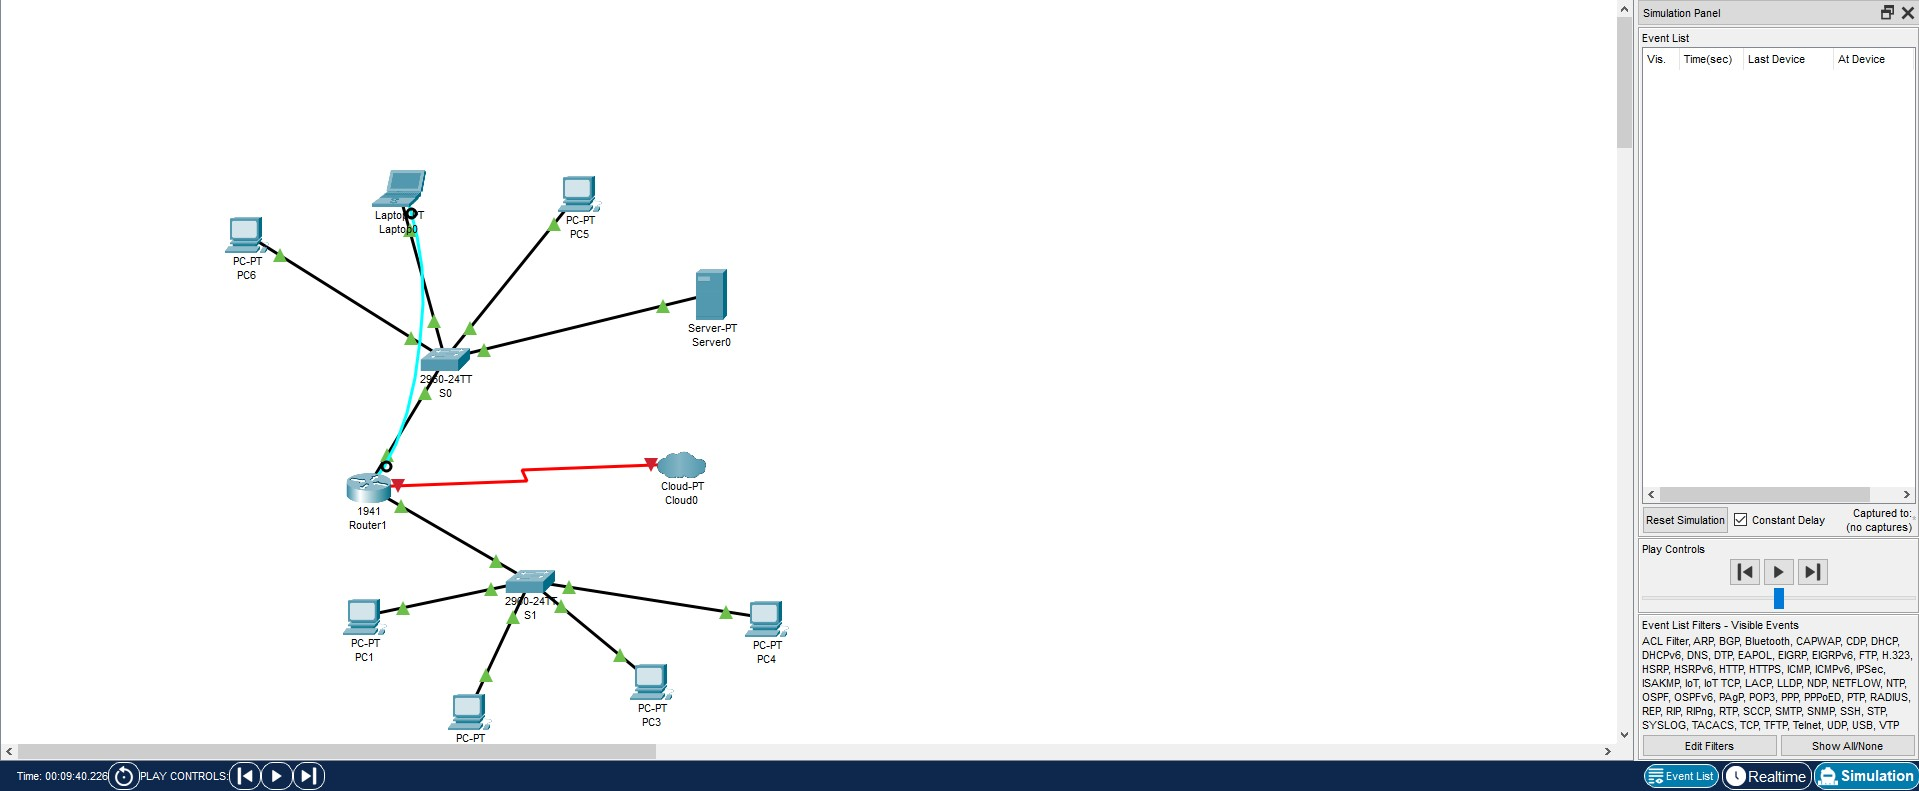
\includegraphics[width=0.75\textwidth]{1}
        \caption{Перевод ПакетТрейсера в режим "Simulation"}
        \label{fig:image1}
    \end{figure}

    \item В окне "Simulation Panel" настройте фильтр событий, отображаемых в ходе симуляции, оставив в списке 
    отображаемых протоколов только ICMP и ARP.

    \begin{figure}[H]
        \centering      %размер рисунка       здесь находится название файла рисунка, без указания формата
        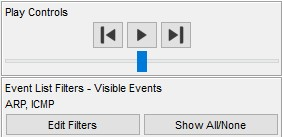
\includegraphics[width=0.75\textwidth]{2}
        \caption{Список отображаемых протоколов}
        \label{fig:image1}
    \end{figure}

    \item Используя инструмент редактирования PDU (протокол дата юнит), сформируйте пакет типа PING для 
    отправки его с компьютера администратора на компьютер в этой же сети. Выбрав режим пошаговой 
    симуляции "Capture/Forvard", выполните полную симуляцию процесса отправки запроса ping до прихода 
    первого ответа.

    \begin{figure}[H]
        \centering      %размер рисунка       здесь находится название файла рисунка, без указания формата
        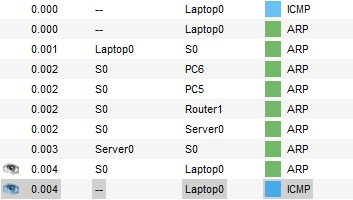
\includegraphics[width=0.75\textwidth]{3}
        \caption{Маршрут пакета}
        \label{fig:image1}
    \end{figure}

    \item Опишите процесс симуляции:
    
    \begin{enumerate}
        \item сколько протоколов участвовало в выполнении запроса: 2
        
        \item какие это были протоколы: ARP, ICMP
        
        \item сколько пакетов было создано и переслано по различным участкам сети: 7
        
        \item приведите мак адреса интерфейсов, через которые проходили ICMP пакеты:
        
        0010.1154.D356

        0060.5C1D.6E68

        0001.C966.92ED

    \end{enumerate}

    \item Используя инструмент редактирования PDU (протокол дата юнит), сформируйте 
    пакет типа PING для отправки его с компьютера администратора на компьютер в другой сети. При 
    этом путь пакета должен проходить через оба маршрутизатора.Выбрав режим пошаговой симуляции 
    "Capture/Forvard", выполните полную симуляцию процесса отправки запроса ping до прихода первого ответа.

    \begin{figure}[H]
        \centering      %размер рисунка       здесь находится название файла рисунка, без указания формата
        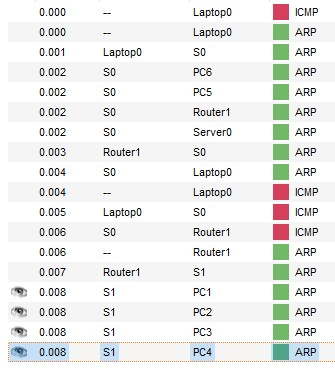
\includegraphics[width=0.75\textwidth]{4}
        \caption{Маршрут пакета}
        \label{fig:image1}
    \end{figure}

    \item Опишите процесс симуляции:
    
    \begin{enumerate}
        \item сколько протоколов участвовало в выполнении запроса: 2
        
        \item какие это были протоколы: ARP, ICMP
        
        \item сколько пакетов было создано и переслано по различным участкам сети: 14
        
        \item приведите мак адреса интерфейсов, через которые проходили ICMP пакеты:
        
        0010.1154.D356

        0060.5C1D.6E68

        0090.21B1.C701

        0090.2124.3153

        0002.4AAD.ED25

    \end{enumerate}

    \item Выбрав режим пошаговой симуляции "Capture/Forvard", повторите полную симуляцию процесса отправки 
    запроса ping в удаленную сеть до прихода первого ответа. Какие протоколы дополнительно появились в 
    списке событий? Для каждого протокола приведите примеры заголовков пакетов всех уровней.

    Новые протоколы не появились.

    \begin{figure}[H]
        \centering      %размер рисунка       здесь находится название файла рисунка, без указания формата
        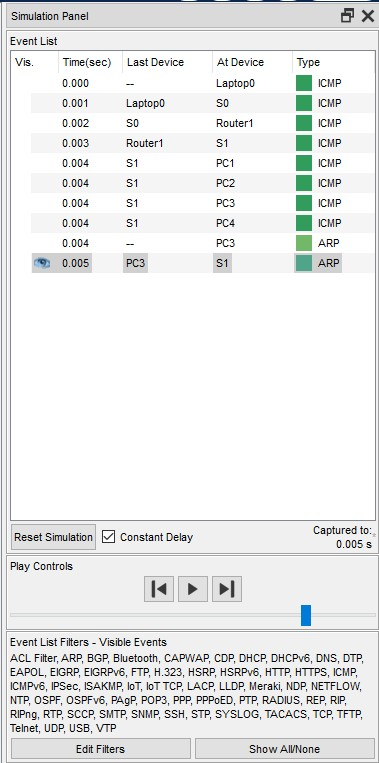
\includegraphics[width=0.6\textwidth]{5}
        \caption{Маршрут пакета}
        \label{fig:image1}
    \end{figure}

    \item Воспользовавшись конфигурационным окном сервера, убедитесь что на нем активен протокол HTTP 
    (закладка "services" окна "config"). Активируйте протокол, если он не активен. На компьютере 
    администратора воспользуйтесь приложением "Web browser" для обращения к HTTP серверу, введя в поле 
    URL IP-адрес сервера и нажав клавишу "Go".

    \begin{figure}[H]
        \centering      %размер рисунка       здесь находится название файла рисунка, без указания формата
        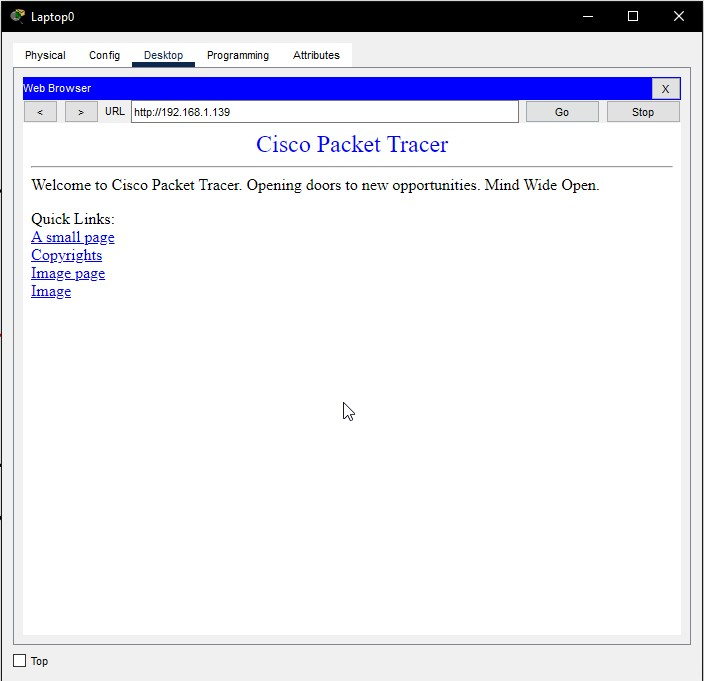
\includegraphics[width=0.75\textwidth]{6}
        \caption{Окно приложения "Web browser"}
        \label{fig:image1}
    \end{figure}
    
    \begin{enumerate}
        \item В ходе симуляции запроса определите протоколы, которые были задействованы: TCP HTTP
        
        \item Сколько пакетов всего было отправлено каждой из сторон: 18
        
        \item Проанализируйте содержание пакетов.
        
        \begin{figure}[H]
            \centering      %размер рисунка       здесь находится название файла рисунка, без указания формата
            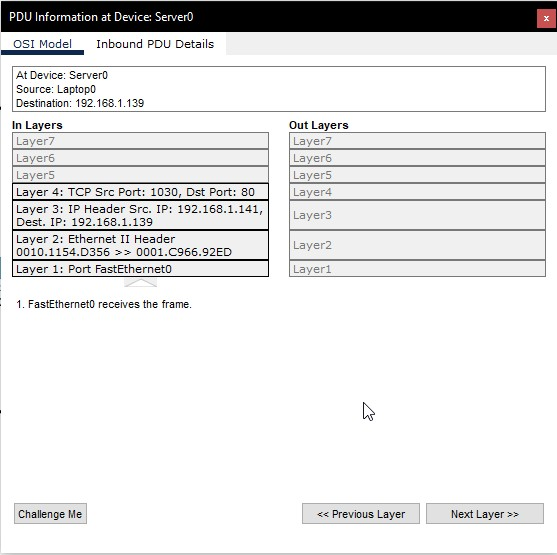
\includegraphics[width=0.75\textwidth]{7}
            \caption{Содержимое пакета}
            \label{fig:image1}
        \end{figure}

        \item Данные каких уровней модели OSI присутствовали в каждом из пакетов: 1 и 2
        
        \item Пошагово опишите процедуру выполнения запроса:
        
        \begin{figure}[H]
            \centering      %размер рисунка       здесь находится название файла рисунка, без указания формата
            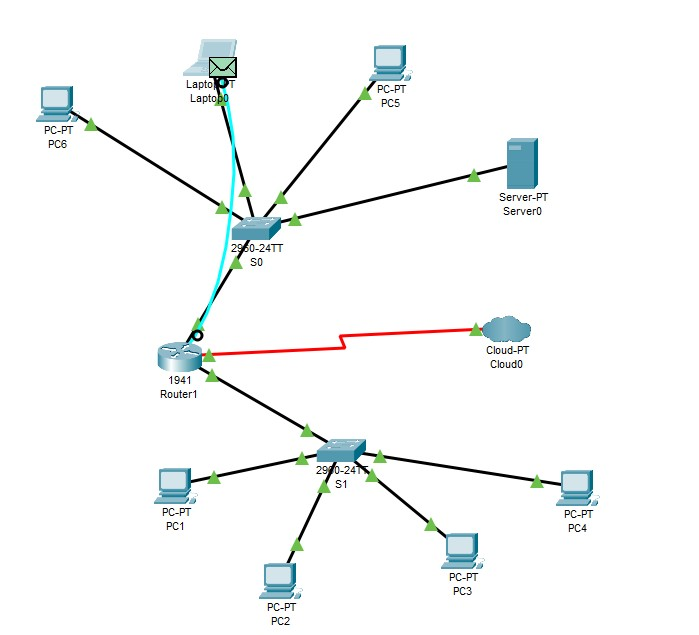
\includegraphics[width=0.6\textwidth]{8}
            \caption{Первый шаг}
            \label{fig:image1}
        \end{figure}

        \begin{figure}[H]
            \centering      %размер рисунка       здесь находится название файла рисунка, без указания формата
            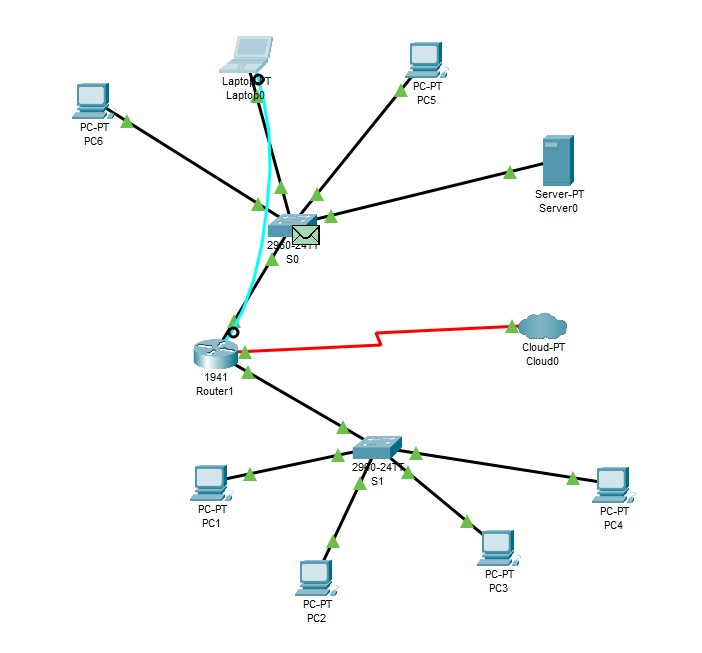
\includegraphics[width=0.6\textwidth]{9}
            \caption{Второй шаг}
            \label{fig:image1}
        \end{figure}

        \begin{figure}[H]
            \centering      %размер рисунка       здесь находится название файла рисунка, без указания формата
            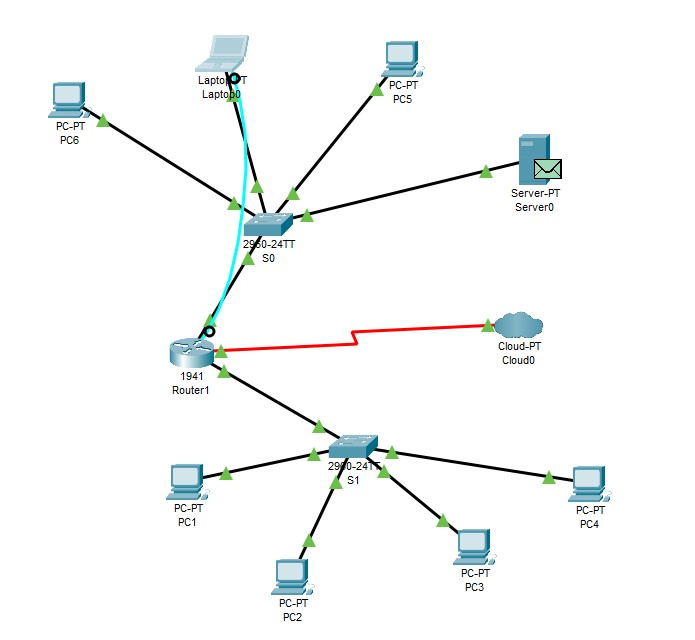
\includegraphics[width=0.6\textwidth]{10}
            \caption{Третий шаг}
            \label{fig:image1}
        \end{figure}

        \begin{figure}[H]
            \centering      %размер рисунка       здесь находится название файла рисунка, без указания формата
            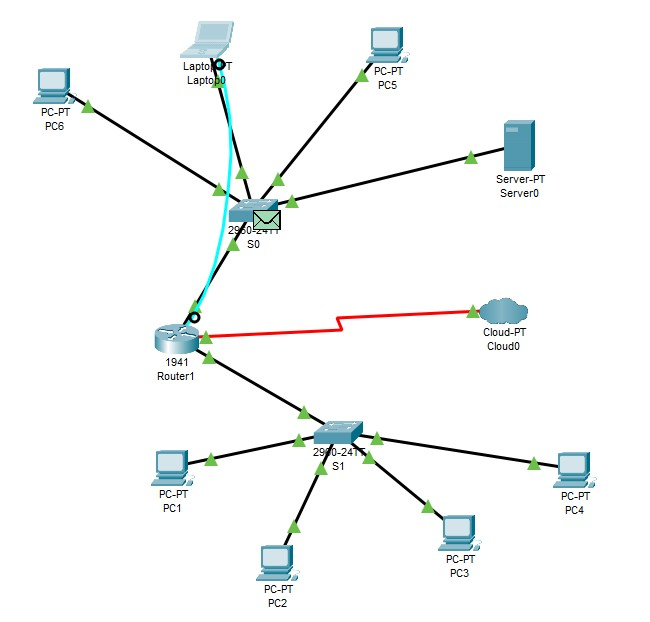
\includegraphics[width=0.6\textwidth]{11}
            \caption{Четвертый шаг}
            \label{fig:image1}
        \end{figure}

        \begin{figure}[H]
            \centering      %размер рисунка       здесь находится название файла рисунка, без указания формата
            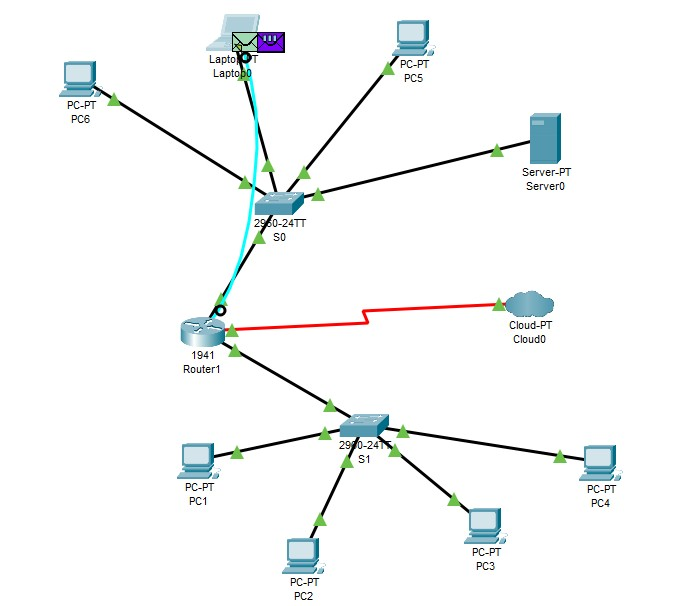
\includegraphics[width=0.6\textwidth]{12}
            \caption{Пятый шаг}
            \label{fig:image1}
        \end{figure}

    \end{enumerate}
\end{enumerate}

\end{document}
